\def\linkdethi{} %Đường link cần dẫn tới
\anmaQR
%%%%%%%%%%%%%%%%%%%%%%%%
\def\toanlop{12}
\def\thoigian{90}
\def\namhoc{2025 - 2026}
\begin{dethi}
	{Bộ GD\&ĐT}
	{VTED ft KING EDU}
	{TDMZD02}
	{Đề thi thử THPTQG 2026}
\end{dethi}
\caulc
\Opensolutionfile{ans}[ans/ansTN-Dung]
%%%=============EX_1=============%%%
\begin{ex}%[1D2N2-4]%[TDMZD02]%[Mui Doan]
	Cho cấp số cộng $(u_n)$ có $u_1=2$ và $d=3$. Giá trị của $u_3$ bằng
	\choice
	{$54$}
	{\True $8$}
	{$11$}
	{$18$}
	\loigiai{
		Ta có $u_3 = u_1 + 2d = 2 + 2\cdot 3 = 8$.
	}
\end{ex}
%%%=============================%%%

%%%=============EX_2=============%%%
\begin{ex}%[1D6H4-2]%[TDMZD02]%[Huỳnh Trí Thiện]
	Nghiệm của phương trình $2^{x+2} = 32$ là
	\choice
	{\True $x=3$}
	{$x=4$}
	{$x=5$}
	{$x=2$}
	\loigiai{
		Ta có $2^{x+2} = 32 \Leftrightarrow 2^{x+2} = 2^5 \Leftrightarrow x+2 = 5 \Leftrightarrow x = 3$.\\
		Vậy nghiệm của phương trình là $x=3$.
	}
\end{ex}
%%%=============================%%%

%%%=============EX_3=============%%%
\begin{ex}%[1D6H4-3]%[TDMZD02]%[Chu Hà]
	Tập nghiệm của bất phương trình $\log\left(x^2-15x\right)<2$ là
	\choice
	{$(-4;25)$}
	{$(21;25)$}
	{$(-5;0)$}
	{\True $(-5;0)\cup(15;20)$}
	\loigiai{
		Điều kiện xác định $x^2-15x>0 \Leftrightarrow \hoac{&x<0\\&x>15.}$\\		
		Bất phương trình đã cho tương đương với
		\[x^2-15x<10^2 \Leftrightarrow x^2-15x-100<0 \Leftrightarrow -5<x<20.\]
		Kết hợp với điều kiện xác định, ta được nghiệm của bất phương trình là $x\in(-5;0)\cup(15;20)$.\\
		Vậy tập nghiệm của bất phương trình là $S=(-5;0)\cup(15;20)$.
	}
\end{ex}
%%%=============================%%%

%%%=============EX_4=============%%%
\begin{ex}%[1H8N2-3]%[TDMZD02]%[Nguyễn Tấn Linh]
	\immini[thm]
	{
		Cho hình chóp đều $S.ABCD$ có tâm của đáy là $O$. Đáp án cho nhận xét \textbf{sai} là
		\choice
		{\True $AD \perp SB$}
		{$SO \perp (ABCD)$}
		{$BD \perp SC$}
		{$BC \perp SO$}
	}
	{
		\begin{tikzpicture}[font=\scriptsize]
			\tikzset{declare function={a=3; b=2; h=2.5;}}
			\path (0,0) coordinate (A)
			(a,0) coordinate (D)
			(-135:b) coordinate (B)
			($(B)+(D)$) coordinate (C)
			($(A)!0.5!(C)$) coordinate (O)
			($(O)+(0,h)$) coordinate (S);
			\path pic[draw,angle radius=6pt]{right angle=A--O--S};
			\path pic[draw,angle radius=6pt]{right angle=D--O--S};
			\draw[dashed] (B)--(A)--(D)--cycle (C)--(A)--(S)--(O);
			\draw (S)--(B)--(C)--(D)--cycle (S)--(C);
			\foreach \t/\g in {A/150,B/-90,C/-60,D/60,S/90,O/-90}{
				\fill (\t) circle (1pt) node[shift={(\g:7pt)},font=\scriptsize]{$\t$};
			}
		\end{tikzpicture}
	}
	\loigiai{
		Vì $S.ABCD$ là hình chóp tứ giác đều có tâm đáy là $O$ nên $ABCD$ là hình vuông và đường cao của hình chóp là $SO$.\\
		Xét từng mệnh đề
		\begin{itemize}
			\item Hình chiếu vuông góc của đường thẳng $SB$ lên mặt phẳng $(ABCD)$ là đường thẳng $OB$. Vì $ABCD$ là hình vuông nên $AD \parallel BC$, do đó góc giữa $AD$ và $OB$ bằng góc giữa $BC$ và $OB$ và bằng $45^\circ$, tức là $AD$ không vuông góc với $OB$. Theo định lí ba đường vuông góc, suy ra $AD$ không vuông góc với $SB$.
			\item Theo tính chất của hình chóp đều, đoạn thẳng nối đỉnh và tâm của đáy chính là đường cao của hình chóp nên $SO \perp (ABCD)$. 
			\item Ta có $BD \perp AC$ (tính chất hai đường chéo hình vuông) và $BD \perp SO$ (do $SO \perp (ABCD)$). Suy ra $BD \perp (SAC)$. Mà $SC \subset (SAC)$ nên $BD \perp SC$.
			\item Vì $SO \perp (ABCD)$ và $BC \subset (ABCD)$ nên $SO \perp BC$ (hay $BC \perp SO$).
		\end{itemize}
	}
\end{ex}
%%%=============================%%%

%%%=============EX_5=============%%%
\begin{ex}%[2D1H2-2]%[TDMZD02]%[Phạm Hải Dương]
	Hàm số $y = x^3 - 24x^2$ đạt cực đại tại điểm
	\choice
	{$x = 16$}
	{\True $x = 0$}
	{$y = 16$}
	{$x = -16$}
	\loigiai{
		Tập xác định $\mathscr{D}=\mathbb{R}$.\\
		Ta có $y' = 3x^2 - 48x$.\\
		Khi đó $y' = 0 \Leftrightarrow 3x^2 - 48x = 0 \Leftrightarrow \hoac{&x = 0 \\ &x = 16.}$\\
		Bảng biến thiên
		\begin{center}
			\begin{tikzpicture}[font=\normalsize,t style/.style={style=solid}]
				\tkzTabInit[nocadre=false,lgt=1.2,espcl=2.5,deltacl=0.5]%,help]
				{$x$/0.75,$y'$/0.75,$y$/3}
				{$-\infty$,$0$,$16$,$+\infty$}
				\tkzTabLine{,+,0,-,0,+}
				\path
				($(N13)!0.1!(N12)$) node (A1){$ -\infty $}
				($(N23)!0.65!(N22)$) node (A2){$ 0 $}
				($(N33)!0.2!(N32)$) node (A3){$ -2\,048 $}
				($(N43)!0.8!(N42)$) node (A4){$ +\infty $};
				\foreach \x/\y in {A1/A2,A2/A3,A3/A4}{
					\draw[-stealth] (\x)--(\y);
				}
			\end{tikzpicture}
		\end{center}
		Từ bảng biến thiên, ta thấy hàm số đạt cực đại tại điểm $x = 0$.
	}
\end{ex}
%%%=============================%%%

%%%=============EX_6=============%%%
\begin{ex}%[1D5H1-3]%[TDMZD02]%[Nguyễn Sơn Thành]
	Cho hai mẫu số liệu ghép nhóm $M_1$, $M_2$ với bảng tần số ghép nhóm như sau
	\begin{center}
		\begin{tabular}{|c|c|c|c|c|c|c|c|}
			\hline
			\multirow{2}{*}{$M_1$} & Nhóm & $[5;7)$ & $[7;9)$ & $[9;11)$ & $[11;13)$ & $[13;15)$ & $[15;17)$\\
			\cline{2-8}
			& Tần số & $3$ & $5$ & $6$ & $4$ & $6$ & $9$\\
			\hline
			\multirow{2}{*}{$M_2$} & Nhóm & $[5;7)$ & $[7;9)$ & $[9;11)$ & $[11;13)$ & $[13;15)$ & $[15;17)$\\
			\cline{2-8}
			& Tần số & $6$ & $10$ & $12$ & $8$ & $12$ & $18$\\
			\hline
		\end{tabular}
	\end{center}
	Gọi $\overline{x}_1$, $\overline{x}_2$ lần lượt là số trung bình cộng của hai mẫu số liệu $M_1$, $M_2$. Đáp án so sánh \textbf{đúng} là
	\choice
	{\True $\overline{x}_1=\overline{x}_2$}
	{$\overline{x}_1<\overline{x}_2$}
	{$\overline{x}_1>\overline{x}_2$}
	{$\overline{x}_1=2\overline{x}_2$}
	\loigiai{
		Chọn giá trị đại diện cho các nhóm dữ liệu, ta có
		\begin{itemize}
			\item Số trung bình cộng của mẫu $M_1$ là\\
			$\overline{x}_1=\dfrac{6 \cdot 3 + 8 \cdot 5 + 10 \cdot 6 + 12 \cdot 4 + 14 \cdot 6 + 16 \cdot 9}{3+5+6+4+6+9}=\dfrac{394}{33}\approx11{,}94$.
			\item Số trung bình cộng của mẫu $M_2$ là\\
			$\overline{x}_2=\dfrac{6 \cdot 6 + 8 \cdot 10 + 10 \cdot 12 + 12 \cdot 8 + 14 \cdot 12 + 16 \cdot 18}{6+10+12+8+12+18}=\dfrac{788}{66}=\dfrac{394}{33}\approx11{,}94$.
		\end{itemize}
		Vậy $\overline{x}_1=\overline{x}_2$.
	}
\end{ex}
%%%=============================%%%

%%%=============EX_7=============%%%
\begin{ex}%[2H2N1-2]%[TDMZD02]%[Bồ Văn Hậu]
	\immini[thm]{Cho hình hộp $ABCD.A'B'C'D'$. Khẳng định nào sau đây là \textbf{đúng}?
		\choice
		{$\overrightarrow{AC}+\overrightarrow{CB'}+\overrightarrow{B'B}=\overrightarrow{AB'}$}
		{$\overrightarrow{AA'}+\overrightarrow{CC'}+\overrightarrow{BB'}=\overrightarrow{AB'}$}
		{\True $\overrightarrow{AC}+\overrightarrow{DD'}+\overrightarrow{C'B'}=\overrightarrow{AB'}$}
		{$\overrightarrow{AB'}+\overrightarrow{B'B}+\overrightarrow{CB'}=\overrightarrow{AB'}$}
	}{
		\begin{tikzpicture}[declare function={a=3; b=0.45*a; h=0.65*a;}]
			\path (0:0) coordinate (A)
			(220:b) coordinate (B)
			($(B)+(a,0)$) coordinate (C)
			(a,0) coordinate (D)
			\foreach \x in {A,B,C,D}{(\x)++(90:h) coordinate (\x1)};
			\draw[dashed] (A1)--(A)--(B)
			(A)--(D);
			\draw (B1)--(A1)--(D1)--(C1)
			(D1)--(D)--(C)
			(B)--(C)--(C1)--(B1)--cycle;
			\foreach \x/\goc/\t in {A/45/A,B/-90/B,C/-90/C,D/0/D,A1/90/A',B1/90/B',C1/90/C',D1/90/D'}
			\fill (\x) circle (1pt) node[shift={(\goc:7pt)},font=\scriptsize]{$\t$};
		\end{tikzpicture}
	}
	\loigiai{
		Xét từng mệnh đề
		\begin{itemize}
			\item Theo quy tắc ba điểm, ta có $\overrightarrow{AC}+\overrightarrow{CB'}+\overrightarrow{B'B} = \left(\overrightarrow{AC}+\overrightarrow{CB'}\right)+\overrightarrow{B'B} = \overrightarrow{AB'} + \overrightarrow{B'B} = \overrightarrow{AB}$.
			\item Vì $ABCD.A'B'C'D'$ là hình hộp nên $\overrightarrow{AA'}=\overrightarrow{BB'}=\overrightarrow{CC'}$. Do đó $\overrightarrow{AA'}+\overrightarrow{CC'}+\overrightarrow{BB'} = 3\overrightarrow{AA'}$. 
			\item Vì $ABCD.A'B'C'D'$ là hình hộp nên $\overrightarrow{DD'}=\overrightarrow{CC'}$. Thay vào biểu thức ta được
			\[\overrightarrow{AC}+\overrightarrow{DD'}+\overrightarrow{C'B'} = \overrightarrow{AC}+\overrightarrow{CC'}+\overrightarrow{C'B'} = \overrightarrow{AC'} + \overrightarrow{C'B'} = \overrightarrow{AB'}.\]	
			\item Theo quy tắc ba điểm, ta có $\overrightarrow{AB'}+\overrightarrow{B'B}+\overrightarrow{CB'} = \left(\overrightarrow{AB'}+\overrightarrow{B'B}\right)+\overrightarrow{CB'} = \overrightarrow{AB} + \overrightarrow{CB'}$. 
		\end{itemize}
		Vậy khẳng định đúng là $\overrightarrow{AC}+\overrightarrow{DD'}+\overrightarrow{C'B'}=\overrightarrow{AB'}$.
	}
\end{ex}
%%%=============================%%%

%%%=============EX_8=============%%%
\begin{ex}%[2D4N1-3]%[TDMZD02]%[Lê Phúc]
	Nếu $C$ là một hằng số thực thì họ nguyên hàm của hàm số $f(x)=\sin x-2\cos x$ là
	\choice
	{$F(x)=\cos x-2\sin x+C$}
	{$F(x)=-\cos x+2\sin x+C$}
	{$F(x)=\sin x-2\cos x+C$}
	{\True $F(x)=-\cos x-2\sin x+C$}
	\loigiai{
		Ta có $F(x)=\displaystyle\int f(x) \mathrm{\,d}x=\displaystyle\int \left(\sin x-2\cos x\right) \mathrm{\,d}x=-\cos x-2\sin x+C$.
	}
\end{ex}
%%%=============================%%%

%%%=============EX_9=============%%%
\begin{ex}%[2H2N2-2]%[TDMZD02]%[Trần Văn Thiện]
	Trong không gian $Oxyz$, cho điểm $A(5;-4;3)$. Điểm đối xứng với $A$ qua trục $Oz$ có tọa độ là 
	\choice
	{\True $(-5;4;3)$}
	{$(-5;-4;3)$}
	{$(5;-4;-3)$}
	{$(0;0;3)$}
	\loigiai{
		Gọi $H$ là hình chiếu vuông góc của điểm $A(5;-4;3)$ lên trục $Oz$, suy ra $H(0;0;3)$.\\
		Gọi $A'$ là điểm đối xứng với $A$ qua trục $Oz$. Khi đó $H$ là trung điểm của đoạn thẳng $AA'$.\\
		Tọa độ điểm $A'$ thỏa mãn
		$\heva{&x_{A'} = 2x_H - x_A = -5 \\ &y_{A'} = 2y_H - y_A = 4 \\ &z_{A'} = 2z_H - z_A = 3} \Rightarrow A'(-5;4;3)$.
	}
\end{ex}
%%%=============================%%%

%%%=============EX_10=============%%%
\begin{ex}%[2D4H3-1]%[TDMZD02]%[Đình Nguyên]
	Diện tích hình phẳng giới hạn bởi các đường $y = x^2 - 3x$, $y = 0$, $x = -1$, $x = 4$ là
	\choice
	{$1$}
	{$\dfrac{4}{3}$}
	{$\dfrac{25}{3}$}
	{\True $\dfrac{49}{6}$}
	\loigiai{
		Phương trình hoành độ giao điểm của đồ thị hàm số $y = x^2 - 3x$ và trục hoành $y = 0$ là
		\[x^2 - 3x = 0 \Leftrightarrow \hoac{&x = 0 \\ &x = 3.}\]
		Các nghiệm $x=0$ và $x=3$ đều thuộc đoạn $[-1; 4]$.\\
		Diện tích hình phẳng cần tìm là
		\allowdisplaybreaks
		\begin{eqnarray*}
			S &=& \displaystyle\int\limits_{-1}^4 |x^2 - 3x| \mathrm{\,d}x  \\
			&=& \displaystyle\int\limits_{-1}^0 |x^2 - 3x| \mathrm{\,d}x + \displaystyle\int\limits_0^3 |x^2 - 3x| \mathrm{\,d}x + \displaystyle\int\limits_3^4 |x^2 - 3x| \mathrm{\,d}x \\
			&=& \displaystyle\int\limits_{-1}^0 (x^2 - 3x) \mathrm{\,d}x - \displaystyle\int\limits_0^3 (x^2 - 3x) \mathrm{\,d}x + \displaystyle\int\limits_3^4 (x^2 - 3x) \mathrm{\,d}x \\
			&=& \left( \dfrac{x^3}{3} - \dfrac{3x^2}{2} \right) \Bigg|_{-1}^0 - \left( \dfrac{x^3}{3} - \dfrac{3x^2}{2} \right) \Bigg|_0^3 +  \left( \dfrac{x^3}{3} - \dfrac{3x^2}{2} \right) \Bigg|_3^4\\
			&=& \dfrac{11}{6} - \left(-\dfrac{9}{2}\right) + \dfrac{11}{6} = \dfrac{49}{6}.
		\end{eqnarray*}
	}
\end{ex}
%%%=============================%%%

%%%=============EX_11=============%%%
\begin{ex}%[2D1H4-3]%[TDMZD02]%[Huynh Quốc Đạt]
	Trong các mệnh đề dưới đây, hỏi có bao nhiêu mệnh đề \textbf{đúng}?
	\begin{enumerate}[1.]
		\item Tiệm cận ngang của một đồ thị $(C)$ luôn không cắt đồ thị $(C)$.
		\item Tiệm cận đứng của một đồ thị $(C)$ có thể có điểm chung với đồ thị $(C)$.
		\item Một đồ thị $(C)$ có tối đa hai đường tiệm cận ngang.
		\item Đồ thị $(C)$ có thể có vô số các đường tiệm cận đứng.
	\end{enumerate}
	\choice
	{\True $3$}
	{$4$}
	{$2$}
	{$1$}
	\loigiai{
		Xét từng mệnh đề
		\begin{itemize}
			\item Ta sẽ lấy phản ví dụ: Vì ta chỉ cần khi biến $x$ tiến tới vô cùng thì đường tiệm cận ngang không cắt đồ thị hàm số, còn với những vị trí khác đồ thị hàm số vẫn có thể cắt tiệm cận ngang, ví dụ như hình vẽ bên dưới.
			\begin{center}
				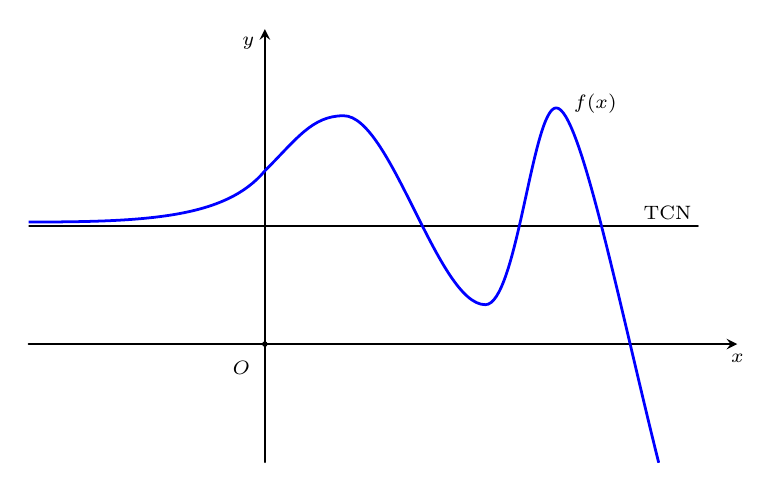
\begin{tikzpicture}[>=stealth,line join=round,line cap=round,every node/.style={font=\scriptsize},declare function={xmin=-3; xmax=6; ymin=-1.5; ymax=4; tcn=1.5;}]
					\draw[-stealth,line width=0.7pt] (xmin,0) -- (xmax,0) node[below] {$x$};
					\draw[-stealth,line width=0.7pt] (0,ymin) -- (0,ymax) node[shift={(-6pt,-5pt)}] {$y$};
					\fill (0,0) circle (1pt) node[shift={(-135:12pt)}] {$O$};
					\begin{scope}
						\clip (xmin,ymin) rectangle (xmax,ymax);
						\draw[line width=0.6pt] (xmin,tcn) -- (5.5,tcn) node[above left,inner sep=2pt] {TCN};
						\draw[blue, line width=1pt] (-3,1.55).. controls (-1.5,1.55) and (-0.5,1.6).. (0,2.2).. controls (0.4,2.6) and (0.6,2.9).. (1,2.9).. controls (1.6,2.9) and (2.2,0.5).. (2.8,0.5).. controls (3.2,0.5) and (3.4,3).. (3.7,3).. controls (4.0,3) and (4.5,0.5).. (5.0,-1.5);
					\end{scope}
					\node[above right] at (3.8,2.8) {$f (x)$};
				\end{tikzpicture}
			\end{center}			
			\item Ta có thể chỉ ra một hàm số (vì tiệm cận đứng là ta chỉ cần xét giới hạn một phía chứ không cần thiết phải giới hạn hai phía). Ví dụ $f(x) = \heva{&2 &&\text{nếu } x \le 1 \\ &\dfrac{1}{x-1} &&\text{nếu } x > 1.}$ \\
			Đồ thị hàm số có tiệm cận đứng là đường thẳng $x=1$, nhưng rõ ràng đường thẳng $x=1$ có điểm chung với đồ thị hàm số là điểm $A(1;2)$ như hình vẽ minh họa bên dưới.
			\begin{center}
				\begin{tikzpicture}[>=stealth, x=1cm, y=1cm, scale=0.8]
					\draw[->] (-3,0) -- (5,0) node[below] {$x$};
					\draw[->] (0,-1) -- (0,4) node[right] {$y$};
					\node[below left] at (0,0) {$O$};
					\draw[dashed, red, thick] (1,-1)node[right] {$x=1$} -- (1,4);
					\draw[blue, thick] (-3,2) -- (1,2);
					\fill[black] (1,2) circle (1.5pt) node[below left] {$A$};
					\node[above left] at (0,2) {$2$};
					\draw[smooth, blue, thick, domain=1.25:4.5, samples=100] plot (\x, {1/(\x-1)}) node[above right] {$(C)$};
				\end{tikzpicture}
			\end{center}			
			\item Đường tiệm cận ngang tồn tại nếu $\hoac{&y_0 = \lim\limits_{x \to +\infty} y \\ &y_0 = \lim\limits_{x \to -\infty} y.}$\\ Suy ra một đồ thị chỉ có tối đa hai đường tiệm cận ngang.
			\item Ví dụ như đồ thị hàm số $y = \tan x$ có vô số đường tiệm cận đứng là $x = \dfrac{\pi}{2} + k\pi$.
		\end{itemize}
		Vậy có tất cả $3$ mệnh đề đúng.
	}
\end{ex}
%%%=============================%%%

%%%=============EX_12=============%%%
\begin{ex}%[2H5H1-3]%[TDMZD02]%[Nguyễn Trí Minh Tuấn]
	Trong không gian $Oxyz$, gọi ba điểm $A$, $B$, $C$ lần lượt là hình chiếu vuông góc của điểm $M(3;2;-2)$ trên các trục $Ox$, $Oy$, $Oz$. Phương trình tổng quát của mặt phẳng $(ABC)$ là
	\choice
	{\True $2x+3y-3z-6=0$}
	{$2x+3y-3z+6=0$}
	{$2x+3y+3z-6=0$}
	{$2x+3y-3z-1=0$}
	\loigiai{
		Vì $A$, $B$, $C$ lần lượt là hình chiếu vuông góc của điểm $M(3;2;-2)$ trên các trục $Ox$, $Oy$, $Oz$ nên ta có tọa độ các điểm là $A(3;0;0)$, $B(0;2;0)$, $C(0;0;-2)$.\\
		Phương trình mặt phẳng $(ABC)$ theo đoạn chắn là
		\[ \dfrac{x}{3}+\dfrac{y}{2}+\dfrac{z}{-2}=1 \Leftrightarrow 2x+3y-3z=6 \Leftrightarrow 2x+3y-3z-6=0. \]
		Vậy phương trình tổng quát của mặt phẳng $(ABC)$ là $2x+3y-3z-6=0$.
	}
\end{ex}
%%%=============================%%%
\Closesolutionfile{ans}

\cauds
\Opensolutionfile{ans}[ans/ansTN-DungSai]
%%%=============EX_13=============%%%
\begin{ex}%[2D4V3-1]%[TDMZD02]%[Dương Công Tạo]
	Hàm số $y = f (x) = ax^3 + bx^2 + cx + d$ có đồ thị $(C)$. Biết $(C)$ có tâm đối xứng là điểm $I(1;3)$ và có một điểm cực trị là $A(-2;5)$.
	\choiceTF[t]
	{\True $3a+b=0$}
	{\True $27a+b+c = 0$}
	{Diện tích hình phẳng giới hạn bởi $(C)$ và đường thẳng $IA$ bằng $\dfrac{1\,070}{153}$}
	{Giá trị nhỏ nhất của hàm số $27x\cdot f (x)-7x$ đạt tại $x = 2$}
	\loigiai{
		\immini{Ta có $f'{(x)} = 3ax^2 + 2bx + c$; $f''{(x)} = 6ax + 2b$.
			\begin{itemize}
				\item Đồ thị ${(C)}$ nhận điểm $I(1;3)$ làm tâm đối xứng nên 
				\[\heva{&f''\left(x_I\right) = 0\\&f{(1)} = 3}\Rightarrow \heva{&3a + b = 0 &&(1)\\&a + b + c + d = 3 &&(2).}\]
				\item Đồ thị ${(C)}$ nhận $A{(-2;5)}$ là điểm cực trị nên 
				\[\heva{&f'(-2) = 0\\&f(-2) = 5}\Rightarrow \heva{&3a\cdot(-2)^2 + 2b\cdot(-2) + c = 0\\&a\cdot(-2)^3 + b\cdot(-2)^2 + c\cdot(-2) + d = 5} \Leftrightarrow \heva{&12a - 4b + c = 0 &&(3)\\&-8a + 4b - 2c + d = 5 &&(4).}\]
			\end{itemize}
			Từ $(1)$, $(2)$, $(3)$, $(4)$ suy ra $\heva{&a = \dfrac{1}{27}\\&b = -\dfrac{1}{9}\\&c = -\dfrac{8}{9}\\&d = \dfrac{107}{27}.}$\\
			Do đó $f{(x)} = \dfrac{1}{27}x^3 - \dfrac{1}{9}x^2 - \dfrac{8}{9}x + \dfrac{107}{27}$.}{
			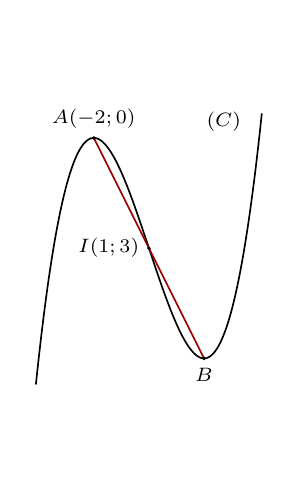
\begin{tikzpicture}[scale=.7,>=stealth,line join=round,line cap=round,every node/.style={font=\scriptsize},declare function={f (\x)=\x^3-3*\x; xmin=-2.2; xmax=2.2; xA=-1; yA=2; xI=0; yI=0; xB=1; yB=-2;}]
				\begin{scope}
					\clip (xmin,-4) rectangle (xmax,4);
					\draw[line width=0.6pt,smooth,samples=300,domain=xmin+0.15:xmax-0.15] plot (\x,{f (\x)});
				\end{scope}
				\draw[line width=0.6pt,red!60!black] (xA,yA) -- (xB,yB);
				\fill (xA,yA) circle (1pt) node[above,font=\scriptsize] {$A (-2; 0)$};
				\fill (xI,yI) circle (1pt) node[left,font=\scriptsize] {$I (1; 3)$};
				\fill (xB,yB) circle (1pt) node[below,font=\scriptsize] {$B$};
				\node[font=\scriptsize, left] at (1.85,2.3) {$(C)$};
		\end{tikzpicture}}
		\begin{itemchoice}
			\itemch Ta có $3a + b = 3\cdot\left( \dfrac{1}{27} \right) + \left( -\dfrac{1}{9} \right)= 0$. 
			\itemch Ta có $27a + b + c=27\cdot\left( \dfrac{1}{27} \right)+ \left( -\dfrac{1}{9} \right)+ \left( -\dfrac{8}{9} \right)= 0$. 
			\itemch Đường thẳng $IA$ đi qua $I(1;3)$ và $A(-2;5)$ có phương trình $y = -\dfrac{2}{3}x + \dfrac{11}{3}$.\\
			Phương trình hoành độ giao điểm của $(C)$ và $IA$ là
			\[\dfrac{1}{27}x^3 - \dfrac{1}{9}x^2 - \dfrac{8}{9}x + \dfrac{107}{27} = -\dfrac{2}{3}x + \dfrac{11}{3}\Leftrightarrow x^3 - 3x^2 - 6x + 8 = 0\Leftrightarrow\hoac{&x=-2\\&x=1\\&x=4.}\]
			Khi đó, diện tích hình phẳng là
			\[S = \displaystyle\int\limits_{-2}^{4} {\left| f(x)- \left( -\dfrac{2}{3}x + \dfrac{11}{3} \right)\right|}\,\mathrm{d}x = \dfrac{1}{27} \displaystyle\int\limits_{-2}^{4} \left| x^3 - 3x^2 - 6x + 8 \right|\,\mathrm{d}x = \dfrac{3}{2} = 1{,}5.\]
			\itemch Xét hàm số $g(x)=27x\cdot f (x)-7x= x^4 - 3x^3 - 24x^2 + 100x$.\\
			Ta có $g'(x)= 4x^3 - 9x^2 - 48x + 100 = (x-2)(4x^2 - x - 50)$.\\
			Khi đó $g'(x)= 0 \Leftrightarrow \hoac{&x = 2 \\ &x = \dfrac{1 \pm 3\sqrt{89}}{8}.}$\\
			Bảng biến thiên
			\begin{center}
				\begin{tikzpicture}[font=\normalsize,t style/.style={style=solid}]
					\tkzTabInit[nocadre=false,lgt=1.2,espcl=2.5,deltacl=0.5]%,help]
					{$x$/1.2,$g'(x)$/0.75,$g (x)$/3}
					{$-\infty$,$\dfrac{1-3\sqrt{89}}{8}$,$2$,$\dfrac{1+3\sqrt{89}}{8}$,$+\infty$}
					\tkzTabLine{,-,0,+,0,+,0,+}
					\path
					($(N13)!0.8!(N12)$) node (A1){$ +\infty $}
					($(N23)!0.1!(N22)$) node (A2){$ \approx -365{,}9$}
					($(N33)!0.7!(N32)$) node (A3){$ 96 $}
					($(N43)!0.3!(N42)$) node (A4){$ \approx 76{,}9 $}
					($(N53)!0.9!(N52)$) node (A5){$ +\infty $};
					\foreach \x/\y in {A1/A2,A2/A3,A3/A4,A4/A5}{
						\draw[-stealth] (\x)--(\y);
					}
				\end{tikzpicture}
			\end{center}
			Khảo sát nhanh ta được giá trị nhỏ nhất của hàm số $g(x)$ đạt tại $x = \dfrac{1-3\sqrt{89}}{8}$.
		\end{itemchoice}	
	}
\end{ex}
%%%=============================%%%

%%%=============EX_14=============%%%
\begin{ex} %[2D4V3-4]%[TDMZD02]%[Hà Văn Hảo]
	\immini[thm]{Cô Yến có một mảnh vườn hình chữ nhật có các kích thước như hình vẽ. Cô Yến dự định sẽ trồng một loại hoa đặc biệt vào phần được gạch chéo giới hạn bởi một parabol $(P)$ có một chiều kích thước bằng $x$ thay đổi được. Biết chi phí trồng hoa là $500$ nghìn đồng tính cho một mét vuông.
		\choiceTF[t]
		{\True Diện tích của mảnh vườn là $300$\,m$^2$}
		{\True Nếu $x = 6$\,m thì diện tích phần trồng hoa sẽ là $60$\,m$^2$}
		{\True Diện tích trồng hoa lớn nhất là $200$\,m$^2$}
		{\True Số tiền dự định trồng hoa là $12$ triệu đồng thì $x = 2{,}4$\,m}
	}{
		\begin{tikzpicture}[>=stealth, x=0.25cm, y=0.25cm]
			\draw[thick, fill=green!10] (0,0) rectangle (15,20);
			\draw[thick, red, fill=white, postaction={pattern=north east lines}] (0,0) parabola bend (7.5,6) (15,0) -- cycle;
			\draw[<->] (0,-1) -- (15,-1) node[midway, below] {$15$\,m};
			\draw[<->] (-1,0) -- (-1,20) node[midway, left] {$20$\,m};
			\draw[<->] (16,0) -- (16,6) node[midway, right] {$x$};
			\node at (10,7) {$(P)$};
		\end{tikzpicture}
	}
	\loigiai{
		\immini{Chọn hệ trục tọa độ $Oxy$ sao cho gốc tọa độ $O$ trùng với góc dưới bên trái của mảnh vườn.\\
			Khi đó, các đỉnh của mảnh vườn hình chữ nhật là $(0;0)$, $(15;0)$, $(15;20)$, $(0;20)$.\\
			Phần trồng hoa được giới hạn bởi trục hoành và đường parabol $(P)$ đi qua các điểm $(0;0)$ và $(15;0)$.\\
			Vì $(P)$ có bề rộng đáy là $15$ và chiều cao là $x$ nên ta có diện tích phần trồng hoa tính theo công thức 
			\[S = \dfrac{2}{3} \cdot 15 \cdot x = 10x.\]
		}{
			\begin{tikzpicture}[>=stealth, x=0.25cm, y=0.25cm]
				\draw[thick, fill=green!10] (0,0) rectangle (15,20);
				\draw[thick, red, fill=white, postaction={pattern=north east lines}] (0,0) parabola bend (7.5,6) (15,0) -- cycle;
				\draw[->] (-1,0) -- (17,0) node[below] {$x$};
				\draw[->] (0,-1) -- (0,22) node[left] {$y$};
				\node (o,0) [below left] {$0$};
				\node at (10,7) {$(P)$};
			\end{tikzpicture}
		}
		\begin{itemchoice}
			\itemch Diện tích mảnh vườn hình chữ nhật là $S_{hcn} = 15 \cdot 20 = 300$\,m$^2$.
			\itemch Với $x = 6$\,m, diện tích phần trồng hoa là $S = 10 \cdot 6 = 60$\,m$^2$. 
			\itemch Vì chiều cao $x$ của parabol không thể vượt quá chiều cao của mảnh vườn là $20$\,m nên diện tích trồng hoa lớn nhất khi $x = 20$\,m.\\
			Khi đó $S_{\max} = 10 \cdot 20 = 200$\,m$^2$.
			\itemch Số tiền dự định trồng hoa là $12\,000\,000$ đồng.\\ Ta có diện tích cần trồng hoa là $12\,000\,000 \colon 500\,000 = 24$\,m$^2$.\\
			Do đó $10x = 24 \Rightarrow x = 2{,}4$\,m.
		\end{itemchoice}
	}
\end{ex}
%%%=============================%%%

%%%=============EX_15=============%%%
\begin{ex}%[2D6V2-4]%[TDMZD02]%[Vũ Hồng Toàn]
	Để kiểm tra chất lượng một máy tự động phát hiện sản phẩm lỗi của một công ty người ta dùng một máy X. Cứ $100$ sản phẩm lỗi thì máy X chỉ thông báo lỗi được $75$ sản phẩm, cứ $100$ sản phẩm không lỗi thì máy X lại thông báo lỗi tới $18$ sản phẩm. Biết rằng tỉ lệ sản phẩm lỗi của công ty đang là $5\%$. Ta tiến hành dùng máy X kiểm tra ngẫu nhiên một sản phẩm. Xét các biến cố: 
	\begin{itemize}
		\item $A$: \lq\lq Sản phẩm được chọn bị lỗi thật\rq\rq, 
		\item $B$: \lq\lq Sản phẩm bị máy X thông báo có lỗi\rq\rq. 
	\end{itemize}
	\choiceTF[t]
	{\True $\mathrm{P}(A)=0{,}05$}
	{\True $\mathrm{P}\left(B\mid A\right)=0{,}75$}
	{\True $\mathrm{P}\left(B\right)=0{,}2085$}
	{\True $\mathrm{P}\left(A\mid B\right)=\dfrac{25}{139}$}
	\loigiai{
		Ta có sơ đồ cây biểu diễn các xác suất như sau
		\begin{center}
			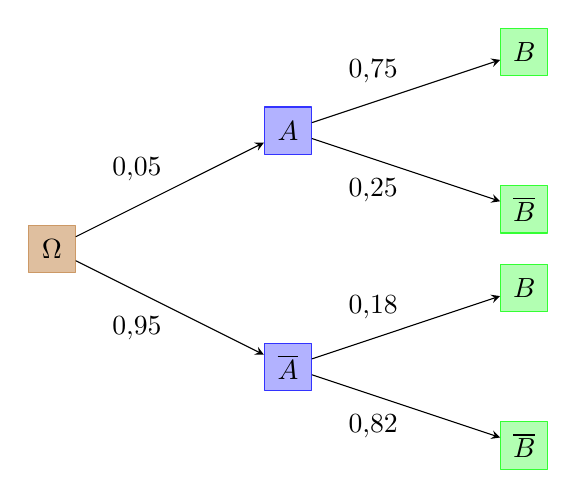
\begin{tikzpicture}[
				line join = round,line cap = round,>=stealth,scale=1,inner sep = 1mm,
				hcnxanh/.style={rectangle,draw = blue!80,fill = blue!30, minimum width=0.6cm, minimum height=0.6cm},
				hcng/.style={rectangle,draw = green!80,fill = green!30, minimum width=0.6cm, minimum height=0.6cm},
				hcnnau/.style={rectangle,draw = brown!80,fill = brown!50, minimum width=0.6cm, minimum height=0.6cm}]
				\node at (0,0) (nodeO) [hcnnau] {$\Omega$};
				\node at (3,1.5) (nodeA) [hcnxanh] {$A$};
				\node at (3,-1.5) (nodeAd) [hcnxanh] {$\overline{A}$};
				\node at (6,2.5) (nodeB1) [hcng] {$B$};
				\node at (6,0.5) (nodeB2) [hcng] {$\overline{B}$};
				\node at (6,-0.5) (nodeB3) [hcng] {$B$};
				\node at (6,-2.5) (nodeB4) [hcng] {$\overline{B}$};
				\draw[->] (nodeO) to node[above left]{$0{,}05$} (nodeA);
				\draw[->] (nodeO) to node[below left]{$0{,}95$} (nodeAd);
				\draw[->] (nodeA) to node[above left]{$0{,}75$} (nodeB1);
				\draw[->] (nodeA) to node[below left]{$0{,}25$} (nodeB2);
				\draw[->] (nodeAd) to node[above left]{$0{,}18$} (nodeB3);
				\draw[->] (nodeAd) to node[below left]{$0{,}82$} (nodeB4);
			\end{tikzpicture}
		\end{center}
		\begin{itemchoice}
			\itemch Tỉ lệ sản phẩm lỗi của công ty là $5\%$, nên $\mathrm{P}\left(A\right) = 0{,}05$. 
			\itemch Cứ $100$ sản phẩm lỗi thì máy X thông báo lỗi được $75$ sản phẩm, nên xác suất máy X thông báo lỗi khi sản phẩm thật sự lỗi là $\mathrm{P}\left(B\mid A\right) = \dfrac{75}{100} = 0{,}75$. 
			\itemch Vì $\mathrm{P}\left(A\right) = 0{,}05\Rightarrow \mathrm{P}\left(\overline{A}\right) = 1 - \mathrm{P}\left(A\right) = 1 - 0{,}05 = 0{,}95$.\\
			Cứ $100$ sản phẩm không lỗi thì máy X thông báo lỗi tới $18$ sản phẩm, nên xác suất máy X thông báo lỗi với điều kiện sản phẩm không lỗi là $\mathrm{P}\left(B\mid \overline{A}\right) = \dfrac{18}{100} = 0{,}18$.\\
			Áp dụng công thức xác suất toàn phần, ta có
			\begin{align*}
				\mathrm{P}\left(B\right) &= \mathrm{P}\left(B\mid A\right)\cdot \mathrm{P}\left(A\right) + \mathrm{P}\left(B\mid \overline{A}\right)\cdot \mathrm{P}\left(\overline{A}\right)\\
				&=0{,}75\cdot 0{,}05 + 0{,}18\cdot 0{,}95\\
				&=0{,}2085.
			\end{align*}			
			\itemch Áp dụng công thức Bayes, ta có
			\begin{align*}
				\mathrm{P}\left(A\mid B\right) &= \dfrac{\mathrm{P}\left(B\mid A\right)\cdot \mathrm{P}\left(A\right)}{\mathrm{P}\left(B\right)}\\
				&=\dfrac{0{,}75 \cdot 0{,}05}{0{,}2085}\\
				&=\dfrac{25}{139}.
			\end{align*}
		\end{itemchoice}
	}
\end{ex}
%%%=============================%%%

%%%=============EX_16=============%%%
\begin{ex}%[2H5V2-5]%[TDMZD02]%[Văn Minh Thoại]
	\immini[thm]{
		Trong không gian $Oxyz$, có một miếng bìa hình tròn $(C)$ chắn được tia sáng không cho đi qua, có bán kính bằng $3$, có tâm là $I(4;1;0)$, nằm trong mặt phẳng $(\alpha)\colon x+2y-6=0$. Một điểm cần quan sát $A(-6;-2;8)$ và mắt người quan sát đặt tại $O$.
	}{
		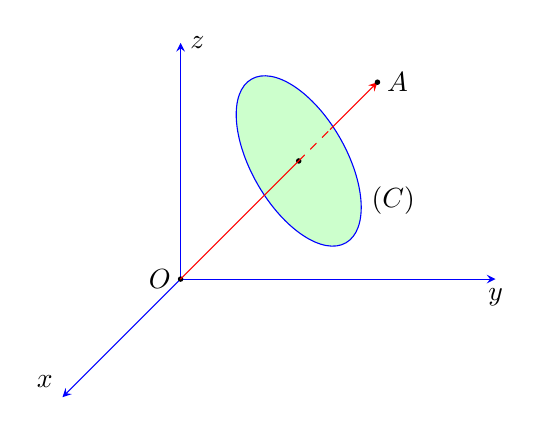
\begin{tikzpicture}[scale=1, >=stealth, line join=round, line cap=round]
			\draw[->, blue] (0, 0) -- (-1.5, -1.5) node[above left, black] {$x$};
			\draw[->, blue] (0, 0) -- (4, 0) node[below, black] {$y$};
			\draw[->, blue] (0, 0) -- (0, 3) node[right, black] {$z$};
			\node at (0, 0) [left] {$O$};
			\fill (0,0) circle (1pt);
			\draw[blue, fill=green!20, rotate around={30:(1.5, 1.5)}] (1.5, 1.5) ellipse (0.6 and 1.2);
			\node at (2.7, 1.0) {$(C)$};
			\fill (1.5,1.5) circle (1pt);
			\draw[red] (0, 0) -- (1.5, 1.5);
			\draw[red, dashed] (1.5, 1.5) -- (1.9, 1.9);
			\draw[->,red] (1.9, 1.9) -- (2.5, 2.5);
			\fill (2.5, 2.5) circle (1pt) node[right] {$A$};
		\end{tikzpicture}
	}
	\choiceTF[t]
	{\True Điểm $M(x;y;z)$ nằm trên $(C)$ thoả mãn $\heva{&(x-4)^2+(y-1)^2+z^2\le 9\\&x+2y-6=0}$}
	{\True Phương trình tham số của đường thẳng $OA$ là $\heva{&x=-6-6t\\&y=-2-2t\\&z=8+8t}$}
	{Nếu đường thẳng $OA$ cắt mặt phẳng $(\alpha)$ tại điểm $N$ thì $IN=\dfrac{\sqrt{195}}{5}$}
	{Người quan sát không nhìn được điểm $A$ vì bị $(C)$ chắn mất tầm nhìn}
	\loigiai{
		\begin{itemchoice}
			\itemch Miếng bìa hình tròn $(C)$ có tâm $I(4;1;0)$ và bán kính $R=3$.\\
			Do đó, các điểm $M(x;y;z)$ thuộc $(C)$ phải nằm trên mặt phẳng $(\alpha)$ và có khoảng cách đến tâm $I$ nhỏ hơn hoặc bằng $R=3$.\\
			Tức là tọa độ điểm $M$ thoả mãn hệ là $\heva{&(x-4)^2+(y-1)^2+z^2\le 9\\&x+2y-6=0}$. 
			\itemch Đường thẳng $OA$ đi qua $A(-6;-2;8)$ và có một vectơ chỉ phương là $\overrightarrow{OA}=(-6;-2;8)$. \\
			Phương trình tham số của đường thẳng $OA$ là $\heva{&x=-6-6t\\&y=-2-2t\\&z=8+8t.}$ 
			\itemch Thay phương trình tham số của đường thẳng $OA$ (ở ý b) vào phương trình mặt phẳng $(\alpha)$, ta có
			\begin{eqnarray*}
				&& (-6-6t) + 2(-2-2t) - 6 = 0\\
				&\Leftrightarrow& -10t - 16 = 0\\ 
				&\Leftrightarrow& t = -\dfrac{8}{5}.
			\end{eqnarray*}
			Suy ra tọa độ điểm giao là $N\left(\dfrac{18}{5};\dfrac{6}{5};-\dfrac{24}{5}\right)$.\\
			Khi đó, khoảng cách $IN$ là
			\[IN=\sqrt{\left(\dfrac{18}{5}-4\right)^2+\left(\dfrac{6}{5}-1\right)^2+\left(-\dfrac{24}{5}-0\right)^2}=\sqrt{\dfrac{4}{25}+\dfrac{1}{25}+\dfrac{576}{25}}=\dfrac{\sqrt{581}}{5}.\]
			\itemch \textbf{Cách 1 (dựa vào vị trí giao điểm):}\\
			Để xác định xem miếng bìa $(C)$ có chắn tầm nhìn từ $O$ đến $A$ hay không, ta cần kiểm tra tia nhìn $OA$ có xuyên qua mặt phẳng $(\alpha)$ tại một điểm nằm trong hình tròn $(C)$ hay không.\\
			Theo chứng minh ở ý c, đường thẳng $OA$ cắt mặt phẳng $(\alpha)$ tại $N$ và có khoảng cách $IN = \dfrac{\sqrt{581}}{5} \approx 4{,}82 > 3 = R$.\\
			Do $IN > R$ nên giao điểm $N$ nằm ngoài hình tròn $(C)$.\\
			Vì vậy, dù mặt phẳng $(\alpha)$ có nằm ngang giữa $O$ và $A$ thì tia nhìn cũng đi ra ngoài rìa miếng bìa.\\ Người quan sát vẫn nhìn thấy điểm $A$ bình thường.\\
			\textbf{Cách 2 (dựa vào vị trí tương đối của điểm và mặt phẳng):}\\
			Xét vị trí tương đối của $O(0;0;0)$ và $A(-6;-2;8)$ đối với mặt phẳng $(\alpha)\colon x+2y-6=0$. \\
			Đặt $f(x;y;z)=x+2y-6$.\\
			Ta có $f(O)=-6<0$ và $f(A)=-6+2\cdot(-2)-6=-16<0$.\\
			Vì $f(O)\cdot f(A)=(-6)\cdot(-16)=96>0$ nên hai điểm $O$ và $A$ nằm về cùng một phía đối với mặt phẳng $(\alpha)$.\\
			Do đó, đoạn thẳng $OA$ hoàn toàn không cắt mặt phẳng $(\alpha)$ chứa miếng bìa.\\ Người quan sát không thể bị miếng bìa chắn tầm nhìn.
		\end{itemchoice}
	}
\end{ex}
%%%=============================%%%
\Closesolutionfile{ans}

\caukq
\Opensolutionfile{ans}[ans/ansTN-DienKhuyet]
%%%=============EX_17=============%%%
\begin{ex}%[1C2H3-1]%[TDMZD02]%[Võ Hiệp]
	\immini[thm]{Một trò chơi điện tử quy định như sau: có $5$ trụ $A$, $B$, $C$, $D$, $E$ với số lượng các thử thách trên đường đi giữa các cặp trụ được mô tả trong hình bên. Người chơi xuất phát từ một trụ nào đó, đi qua tất cả các trụ còn lại, mỗi lần đi qua một trụ thì trụ đó sẽ bị phá hủy và không thể quay trở lại trụ đó được nữa, nhưng người chơi vẫn phải quay trở về trụ ban đầu. Tổng số thử thách của đường đi thỏa mãn điều kiện trên nhận giá trị nhỏ nhất là bao nhiêu?
	}{
		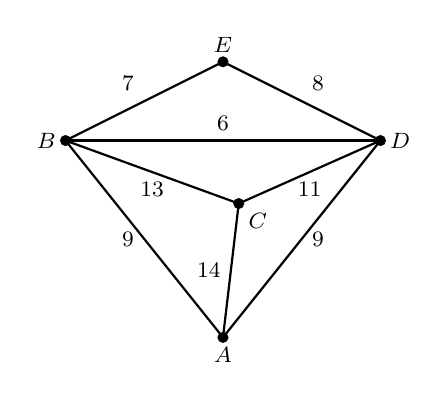
\begin{tikzpicture}[scale=1, font=\footnotesize, line join=round, line cap=round, >=stealth]
			% Tọa độ các trụ
			\coordinate (A) at (2,-2.5);
			\coordinate (B) at (0,0);
			\coordinate (C) at (2.2,-0.8);
			\coordinate (D) at (4,0);
			\coordinate (E) at (2,1);
			
			% Vẽ các cạnh và ghi nhãn trọng số
			\draw[thick] (B)--(E) node[midway, above left] {7};
			\draw[thick] (E)--(D) node[midway, above right] {8};
			\draw[thick] (B)--(D) node[midway, above] {6};
			\draw[thick] (B)--(C) node[midway, below] {13};
			\draw[thick] (C)--(D) node[midway, below] {11};
			\draw[thick] (B)--(A) node[midway, left] {9};
			\draw[thick] (C)--(A) node[midway, left] {14};
			\draw[thick] (D)--(A) node[midway, right] {9};
			
			% Vẽ các trụ (chấm tròn) và ghi nhãn
			\foreach \point/\labelpos in {A/below, B/left, C/below right, D/right, E/above} {
				\fill (\point) circle (2pt);
				\node[\labelpos] at (\point) {$\point$};
			}
		\end{tikzpicture}
	}
	\par	
	\shortans[0]{49}
	\loigiai{
		Một đường đi thoả mãn đi qua tất cả các đỉnh, mỗi đỉnh một lần, khi đó mỗi đỉnh sẽ nối với đúng hai cạnh, một cạnh đi đến đỉnh và một cạnh ra khỏi đỉnh. Trong một chu trình thì ta bắt đầu đi từ đỉnh nào cũng được. Chính vì vậy, ta sẽ chọn đỉnh bắt đầu đi (cũng là đỉnh kết thúc) là đỉnh nối với số cạnh ít nhất. Như ở bài toán này thì ta chọn đỉnh $E$. Ta có các trường hợp sau:
		\begin{center}
			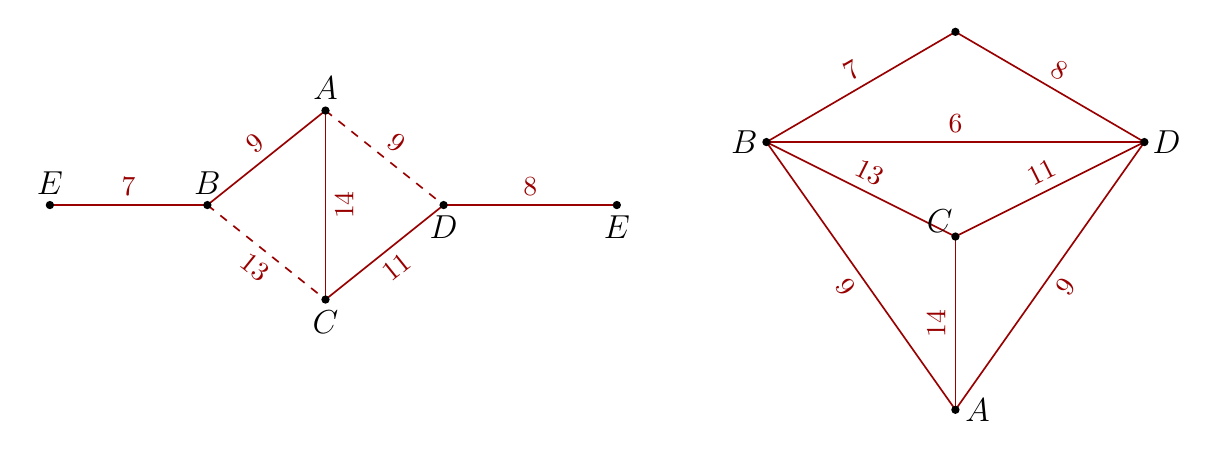
\begin{tikzpicture}[declare function={shiftX=6.5;}]
				\tikzset{
					edge/.style={line width=0.6pt,color=red!60!black},
					dashed edge/.style={line width=0.6pt,dashed,color=red!60!black}
				}
				\path
				(-5,0) coordinate (El)
				(-3,0) coordinate (Bl)
				(-1.5,1.2) coordinate (Al)
				(-1.5,-1.2) coordinate (Cl)
				(0,0) coordinate (Dl)
				(2.2,0) coordinate (Er)
				(shiftX,2.2) coordinate (Et)
				(shiftX - 2.4,0.8) coordinate (Br)
				(shiftX + 2.4,0.8) coordinate (Dr)
				(shiftX,-0.4) coordinate (Cr)
				(shiftX,-2.6) coordinate (Ar);
				\draw[edge] (El) -- (Bl) node[pos=0.5,sloped,above] {$7$};
				\draw[edge] (Bl) -- (Al) node[pos=0.5,sloped,above] {$9$};
				\draw[dashed edge] (Bl) -- (Cl) node[pos=0.5,sloped,below] {$13$};
				\draw[edge] (Cl) -- (Al) node[pos=0.5,sloped,below] {$14$};
				\draw[dashed edge] (Al) -- (Dl) node[pos=0.5,sloped,above] {$9$};
				\draw[edge] (Cl) -- (Dl) node[pos=0.5,sloped,below] {$11$};
				\draw[edge] (Dl) -- (Er) node[pos=0.5,sloped,above] {$8$};
				\draw[edge] (Br) -- (Et) node[pos=0.5,sloped,above] {$7$};
				\draw[edge] (Et) -- (Dr) node[pos=0.5,sloped,above] {$8$};
				\draw[edge] (Br) -- (Dr) node[pos=0.5,sloped,above] {$6$};
				\draw[edge] (Br) -- (Cr) node[pos=0.5,sloped,above] {$13$};
				\draw[edge] (Cr) -- (Dr) node[pos=0.5,sloped,above] {$11$};
				\draw[edge] (Br) -- (Ar) node[pos=0.5,sloped,below] {$9$};
				\draw[edge] (Ar) -- (Dr) node[pos=0.5,sloped,below] {$9$};
				\draw[edge] (Ar) -- (Cr) node[pos=0.5,sloped,above] {$14$};
				\foreach \p/\pos/\text in {
					El/90/E,Bl/90/B,Al/90/A,Cl/-90/C,Dl/-90/D,Er/-90/E,
					Br/180/B,Dr/0/D,Cr/135/C,Ar/0/A
				}{
					\fill (\p) circle (1.5pt);
					\draw (\p) circle (0.6pt) node[shift={(\pos:8pt)},font=\large] {$\text$};
				}
				\fill (Et) circle (1.5pt);
				\draw (Et) circle (0.6pt);
			\end{tikzpicture}
		\end{center}
		\begin{itemize}
			\item Sơ đồ $1$: $E \xrightarrow{\,7\,} B \xrightarrow{\,9\,} A \xrightarrow{\,14\,} C \xrightarrow{\,11\,} D \xrightarrow{\,8\,} E$.
			\item Sơ đồ $2$: $E \xrightarrow{\,7\,} B \xrightarrow{\,13\,} C \xrightarrow{\,14\,} A \xrightarrow{\,9\,} D \xrightarrow{\,8\,} E$.
		\end{itemize}
		Sơ đồ $1$ ngắn hơn với tổng thử thách bằng $7+9+14+11+8=49$.\\
		Vậy tổng số thử thách nhận giá trị nhỏ nhất là $49$.
	}
\end{ex}
%%%=============================%%%

%%%=============EX_18=============%%%
\begin{ex}%[1H8V7-4]%[TDMZD02]%[Duong Xuan Loi]
	Cho lăng trụ $ABC.A'B'C'$ có đáy $ABC$ là tam giác với $AB=AC=6$. Biết hình chiếu vuông góc của $A$ và $C$ lên cạnh $A'B'$ trùng nhau, khoảng cách từ $A$ và $C$ đến $A'B'$ đều bằng $8$. Hãy tính thể tích khối lăng trụ $ABC.A'B'C'$ (\textit{làm tròn kết quả đến hàng đơn vị}).
	\par
	\shortans[0]{133}
	\loigiai{
		\immini{Gọi $H$ là hình chiếu vuông góc của $A$ và $C$ lên cạnh $A'B'$.\\
			Suy ra tam giác $HAC$ là tam giác cân tại $H$ và có $HA = HC = 8$; $AC = 6$.\\
			Ta có $\heva{& A'B' \perp HA \\ & A'B' \perp HC} \Rightarrow A'B' \perp (HAC)$.\\
			Vì $AC \subset (HAC)$ nên $A'B' \perp AC$.\\
			Mặt khác, $AB \parallel A'B'$ (tính chất lăng trụ) $\Rightarrow AB \perp AC \Rightarrow \triangle ABC$ vuông tại $A$.\\
			Gọi $K$ là trung điểm của $AC$.}{
			\begin{tikzpicture}[scale=1, font=\footnotesize, line join=round, line cap=round,>=stealth]
				\path
				(0,0)coordinate (A)
				(2.5,-1.5)coordinate (B)
				(4,0)coordinate (C)
				($(C)!0.5!(A)$) coordinate (K)	
				($(A)+(1,3.2)$) coordinate (A')
				($(A')+(B)-(A)$)coordinate (B')
				($(A')+(C)-(A)$)coordinate (C')		
				($(A')!0.4!(B')$) coordinate (H)										
				;
				\draw (A)--(B)--(C)--(C')--(B')--(A')--cycle (A')--(C') (B)--(B') (A)--(H);
				\draw[dashed] (A)--(C)--(H)--(K);	
				\foreach \p/\q in {A/180,B/-90,C/0,A'/180,B'/75,C'/0,H/60,K/-90}
				\fill[black] (\p) circle (1.0pt)node[shift={(\q:3mm)}]{$\p$};
			\end{tikzpicture}
		} 
		Suy ra
		\begin{itemize}
			\item Vì $\triangle HAC$ cân tại $H$ nên đường trung tuyến $HK$ đồng thời là đường cao $\Rightarrow HK \perp AC$.
			\item Vì $A'B' \perp (HAC)$ và $HK \subset (HAC)$ nên $A'B' \perp HK \Leftrightarrow AB \perp HK$.
		\end{itemize}
		Từ $\heva{& HK \perp AC \\ & HK \perp AB} \Rightarrow HK \perp (ABC)$.\\
		Do đó, $HK$ là đường cao của lăng trụ và cũng là khoảng cách giữa hai mặt đáy.\\
		Xét $\triangle HAK$ vuông tại $K$, ta có $AK = \dfrac{AC}{2} = 3$.\\
		Suy ra $HK = \sqrt{HA^2 - AK^2} = \sqrt{8^2 - 3^2} = \sqrt{55}$.\\
		Thể tích của khối lăng trụ $ABC.A'B'C'$ là
		\[ V_{ABC.A'B'C'} = S_{\triangle ABC} \cdot HK = \left( \dfrac{1}{2} \cdot AB \cdot AC \right) \cdot HK = \dfrac{1}{2} \cdot 6 \cdot 6 \cdot \sqrt{55} = 18\sqrt{55} \approx 133{,}49 \approx 133. \]
	}
\end{ex}
%%%=============================%%%

%%%=============EX_19=============%%%
\begin{ex}%[2H2V2-6]%[TDMZD02]%[Nguyễn Đức Tuấn Anh]
	Tiến hành gắn hệ trục toạ độ $Oxyz$ vào một căn phòng triển lãm, với đơn vị dài trên mỗi trục toạ độ là $160$\,cm. Một người đứng tại một vị trí mà toạ độ của mắt người đó là $M(1;0;1)$. Người này tiến hành quan sát hai quả cầu phong thuỷ đá quý I và II thì cảm thấy rằng chúng to bằng nhau, quả cầu I có tâm tại $A(4;3;1)$, quả cầu II có tâm tại $B(0;2;2)$. Biết rằng quả cầu I có thể tích bằng $90$\,dm$^3$ và quả cầu II có thể tích không vượt quá $120$\,dm$^3$. Hãy xác định thể tích quả cầu II theo đơn vị dm$^3$ (\textit{làm tròn kết quả đến hàng phần mười}).
	\begin{center}
		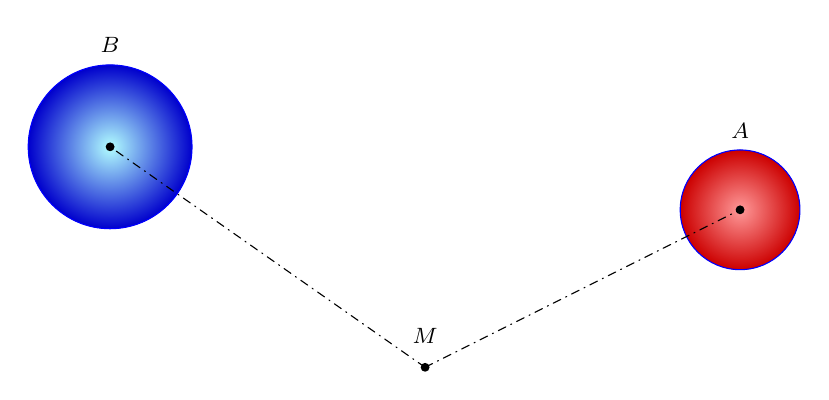
\begin{tikzpicture}[scale=.8, font=\footnotesize, line join=round, line cap=round, >=stealth]
			\path (5,0) coordinate (M) (0,3.5) coordinate (B) (10,2.5) coordinate (A);
			\fill[shading=radial,inner color=cyan!30!white,outer color=blue!80!black] (B) circle (1.3);
			\draw[blue] (B) circle (1.3);
			\fill[shading=radial,inner color=red!40!white,outer color=red!80!black] (A) circle (0.95);
			\draw[blue] (A) circle (0.95);
			\draw[dash dot] (M)--(B) (M)--(A);
			\foreach \p/\ang/\dist/\lbl in {M/90/0.4/M, B/90/1.3/B, A/90/1/A} \fill (\p) circle (2pt) node[shift={(\ang:\dist)}] {$\lbl$};
		\end{tikzpicture}
	\end{center}
	\par
	\shortans[0]{90,5}
	\loigiai{
		Ta chấp nhận kết quả: \lq\lq Người quan sát nhìn thấy quả cầu to hay nhỏ dựa vào kích thước của bán kính đường tròn lớn nhất (gọi là bán kính ngắm) mà người đó nhìn thấy được từ điểm quan sát đến quả cầu.\rq\rq
		\begin{center}
			\begin{tikzpicture}[
				declare function={
					R=2.5;
					d=6.25;
					xH=-R*R/d;
					rC=R*sqrt (d*d-R*R)/d;
					rx=0.6;
				},
				>=stealth,
				line join=round,
				line cap=round,
				every node/.style={font=\scriptsize}
				]
				\path
				(0,0) coordinate (A)
				(-d,0) coordinate (M)
				(xH,0) coordinate (H)
				(xH,rC) coordinate (E)
				(xH,-rC) coordinate (F);
				\draw[line width=0.6pt] (A) circle (R);
				\draw[line width=0.6pt] (M) -- ($(M)!1.3!(E)$);
				\draw[line width=0.6pt] (M) -- ($(M)!1.3!(F)$);
				\draw[line width=0.6pt,red!60!black] plot[domain=-90:90,samples=100] ({xH + rx*cos (\x)},{rC*sin (\x)});
				\draw[line width=0.6pt,red!60!black,dash pattern=on 2pt off 1.5pt] plot[domain=90:270,samples=100] ({xH + rx*cos (\x)},{rC*sin (\x)});
				\draw[line width=0.6pt,dash pattern=on 2pt off 1.5pt] (M) -- (A);
				\draw[line width=0.6pt,dash pattern=on 2pt off 1.5pt] (E) -- (F);
				\path (H) -- (E) node[midway,left=1pt] {$r$};
				\node[shift={(105:10pt)}] at (E) {$E$};
				\node at (320:3.2) {$(S)$};
				\foreach \p/\pos in {M/-135,A/0,H/-120}{
					\draw (\p) circle (0.6pt) node[shift={(\pos:8pt)},font=\scriptsize] {$\p$};
				}
			\end{tikzpicture}
		\end{center}
		Xét mặt phẳng chứa điểm ngắm $M$ và tâm $A$ của quả cầu bán kính $R$.\\ Kẻ các tiếp tuyến từ $M$ đến đường tròn lớn tâm $A$, các tiếp điểm sẽ chạy quanh $MA$ tạo thành một đường tròn ngắm. \\
		Gọi $E$ là một tiếp điểm và $H$ là hình chiếu vuông góc của $E$ lên trục $MA$.\\ Bán kính ngắm của quả cầu khi đó chính là đoạn $r = HE$.\\
		Trong tam giác vuông $MEA$ tại $E$, có đường cao $EH$.\\ Áp dụng hệ thức lượng, ta có $HE = AE \cos \widehat{AEH}$. \\
		Do hai góc $\widehat{AEH}$ và $\widehat{AME}$ có cạnh tương ứng vuông góc nên $\widehat{AEH} = \widehat{AME}$, suy ra $r = R \cos \widehat{AME}$.\\
		Mặt khác, $\sin \widehat{AME} = \dfrac{AE}{MA} = \dfrac{R}{MA}$.\\ Từ đó $\cos \widehat{AME} = \sqrt{1 - \sin^2 \widehat{AME}} = \sqrt{1 - \dfrac{R^2}{MA^2}}$.\\
		Suy ra công thức tính bán kính ngắm một quả cầu là $r = R \sqrt{1 - \dfrac{R^2}{MA^2}} = \sqrt{R^2 - \dfrac{R^4}{MA^2}}$.\\
		Người quan sát đứng tại $M$ ngắm hai quả cầu I (tâm $A$) và II (tâm $B$) thấy to bằng nhau, đồng nghĩa với việc bán kính ngắm của hai quả cầu bằng nhau: $r_A = r_B \Leftrightarrow R_A^2 - \dfrac{R_A^4}{MA^2} = R_B^2 - \dfrac{R_B^4}{MB^2} \quad (1)$.\\
		Tính khoảng cách từ $M$ đến tâm các quả cầu trong hệ tọa độ $MA = \sqrt{(4-1)^2 + 3^2 + (1-1)^2} = 3\sqrt{2}$ và $MB = \sqrt{(0-1)^2 + 2^2 + (2-1)^2} = \sqrt{6}$.\\
		Tiến hành quy đổi đơn vị: $1$ đơn vị chiều dài trên hệ trục toạ độ tương ứng với $160$\,cm $= 16$\,dm.\\
		Thể tích quả cầu I thực tế là $V_A = 90$\,dm$^3$, nên bán kính thực tế của quả cầu I là \[R_{A'} = \sqrt[3]{\dfrac{3V_A}{4\pi}} \approx 2{,}7797\,\text{dm}.\]
		Quy đổi ngược vào hệ tọa độ, bán kính quả cầu I là $R_A = \dfrac{2{,}7797}{16} \approx 0{,}1737$.\\
		Thay các giá trị $MA$, $MB$ và $R_A$ vào phương trình $(1)$, ta có \[0{,}1737^2 - \dfrac{0{,}1737^4}{\left(3\sqrt{2}\right)^2} = R_B^2 - \dfrac{R_B^4}{\left(\sqrt{6}\right)^2} \Leftrightarrow R_B^2 - \dfrac{R_B^4}{6} \approx 0{,}03013.\]
		Đặt $t = R_B^2$ ($t > 0$), phương trình trở thành $\dfrac{t^2}{6} - t + 0{,}03013 = 0 \Leftrightarrow t^2 - 6t + 0{,}18078 = 0$.\\
		Giải phương trình bậc hai trên, ta thu được hai nghiệm $t \approx 5{,}9697$ hoặc $t \approx 0{,}03029$.\\
		\textbf{Trường hợp 1:} Nếu $R_B^2 \approx 5{,}9697 \Rightarrow R_B \approx 2{,}4433$.\\ Bán kính thực tế của quả cầu II là $R_{B'} = R_B \cdot 16 \approx 39{,}09$\,dm.\\ Thể tích khi đó là $V_B = \dfrac{4}{3}\pi R_{B'}^3 \approx 250326$\,dm$^3$ (loại vì giả thiết thể tích không vượt quá $120$\,dm$^3$).\\
		\textbf{Trường hợp 2:} Nếu $R_B^2 \approx 0{,}03029 \Rightarrow R_B \approx 0{,}17404$.\\ Bán kính thực tế của quả cầu II là $R_{B'} = R_B \cdot 16 \approx 2{,}7847$\,dm.\\ Thể tích khi đó là $V_B = \dfrac{4}{3}\pi R_{B'}^3 \approx 90{,}4578$\,dm$^3 \approx 90{,}5$\,dm$^3$ (thỏa mãn).\\
		Vậy thể tích của quả cầu II xấp xỉ $90{,}5$\,dm$^3$.
	}
\end{ex}
%%%=============================%%%

\begin{ex}
	\sochc{2}
	Cho ba thanh cứng $AB$, $BC$, $CD$ gắn với nhau bằng hai bản lề tại $B$ và $C$, hai đầu còn lại được gắn cố định với sàn nhà tại hai bản lề $A$ và $D$. Biết rằng $AB=CD=5$\,m, $BC=3$\,m, $AD=6$\,m, mặt phẳng $(ABCD)$ luôn vuông góc với sàn nhà.
	\begin{center}
		\begin{tikzpicture}[scale=0.8, line join=round, line cap=round, >=stealth, font=\footnotesize]
			\def\h{4}
			\coordinate (H) at (0,0);
			\coordinate (C) at (0,\h);
			\coordinate (D) at (-3,0);
			\coordinate (B) at (4,\h);
			\coordinate (A) at (6,0);
			\draw (-6,0) -- (10,0);
			\node[above] at (9,0) {Sàn nhà};
			\draw[very thick, red!80!black] (D) -- (C) node[midway, left, black] {$5\,m$};
			\draw[very thick, blue!60!black] (C) -- (B) node[midway, below, black] {$3\,m$};
			\draw[very thick, blue] (B) -- (A) node[midway, right, black] {$5\,m$};
			\draw[dashed] (C) -- (H) node[midway, left] {$h$};
			\draw (C) -- (A);
			\foreach \p/\pos in {D/above left, H/below, A/above right, C/above, B/above} {
				\filldraw[blue, draw=black] (\p) circle (2pt);
				\node[\pos] at (\p) {\p};
			}
			\node[below, yshift=-2pt] at (D) {Cố định};
			\node[below, yshift=-2pt] at (A) {Cố định};
			
		\end{tikzpicture}
	\end{center}
	
	%%%=============EX_20=============%%%
	\begin{chc}%[0H4V3-2]%[TDMZD02]%[Dự án đề thi]
		Khi hai bản lề $B$ và $C$ di chuyển thì điểm $C$ cách sàn nhà một khoảng ngắn nhất bằng bao nhiêu cm \textit{(làm tròn kết quả đến hàng đơn vị)}?
		\par
		\shortans[0]{156}
		\loigiai{
			Gọi $h$ là khoảng cách từ $C$ đến sàn nhà $AD$.\\ 
			Kẻ $CH \perp AD$ tại $H$.\\
			Xét tam giác $ACH$ vuông tại $H$, ta có $AC^2 = AH^2 + CH^2 = (AD - DH)^2 + h^2$.\\
			Do $DH = \sqrt{CD^2 - CH^2} = \sqrt{25 - h^2}$ nên suy ra
			\[AC^2 = \left(6 - \sqrt{25 - h^2}\right)^2 + h^2 = 36 - 12\sqrt{25 - h^2} + 25 - h^2 + h^2 = 61 - 12\sqrt{25 - h^2}.\]
			Dễ thấy khi khoảng cách $h$ giảm thì $\sqrt{25 - h^2}$ tăng, kéo theo $AC^2 = 61 - 12\sqrt{25 - h^2}$ giảm.\\ Như vậy, khoảng cách $h$ đạt giá trị nhỏ nhất khi độ dài $AC$ nhỏ nhất.\\
			Áp dụng bất đẳng thức tam giác cho bộ ba điểm $A$, $B$, $C$ ta luôn có
			\[AC \ge |AB - BC| = |5 - 3| = 2 \Rightarrow AC_{\min} = 2.\]
			Khi đó, ta có phương trình
			\[2^2 = 61 - 12\sqrt{25 - h_{\min}^2} \Leftrightarrow 12\sqrt{25 - h_{\min}^2} = 57 \Leftrightarrow \sqrt{25 - h_{\min}^2} = \dfrac{19}{4}.\]
			Bình phương hai vế ta được
			\[25 - h_{\min}^2 = \dfrac{361}{16} \Leftrightarrow h_{\min}^2 = \dfrac{39}{16} \Rightarrow h_{\min} = \dfrac{\sqrt{39}}{4} \approx 1{,}5612 \text{ (m)}.\]
			Đổi $1{,}5612$\,m $= 156{,}12$\,cm.\\ 
			Làm tròn đến hàng đơn vị, khoảng cách ngắn nhất là $156$\,cm.
		}
	\end{chc}
	%%%=============================%%%
	
	%%%=============EX_21=============%%%
	\begin{chc}%[2D4V3-4]%[TDMZD02]%[Nguyễn Văn Sang]
		Khi hai bản lề $B$ và $C$ di chuyển thì $AB$, $CD$ lần lượt quét thành các hình phẳng $(H_1)$, $(H_2)$. Gọi $(H) = (H_1) \cap (H_2)$. Hãy tính diện tích của $(H)$ theo đơn vị mét vuông (\textit{làm tròn kết quả đến hàng phần mười}).
		\par
		\shortans[0]{6,2}
		\loigiai{
			\begin{center}
				\begin{tikzpicture}[declare function={r=3;},line cap=round,line join=round,font=\footnotesize,>=stealth]
					\def\xmin{-2}\def\xmax{7}\def\ymin{-1}\def\ymax{4}
					\draw[->](\xmin,0)--(\xmax,0) node[below]{$x$};
					\draw[->](0,\ymin)--(0,\ymax) node[left]{$y$};
					\foreach \x/\y in {C_2/20,M/40,C/60,C_1/120}{\path
						(\y:r) coordinate (\x);}
					\path (0,0) coordinate (O)
					(O)++(0:0.5) coordinate (Z)
					($(O)!(C_2)!(Z)$) coordinate (Z1)
					($(O)!(M)!(Z1)$) coordinate (N)
					($(O)!2!(N)$) coordinate (A)
					(A)++(120:0.8*r) coordinate (B)
					($(O)!(C)!(Z1)$) coordinate (H);
					\foreach \x/\y in {O/C_2,O/M,O/C,O/C_1}{
						\draw (\x)--(\y);
					}
					\foreach \x/\y in {B_1/60,B_2/160}{
						\path (A)++(\y:r) coordinate (\x);
					}
					\foreach \x/\y in {A/B_1,A/B_2,A/B,A/C}{
						\draw (\x)--(\y);
					}
					\draw (20:r) arc[start angle=20,end angle=120,radius=r];
					\draw (A)++(60:r) arc[start angle=60,end angle=160,radius=r];
					\draw[dashed](M)--(N)
					(C)--(H)
					(C_2)--(Z1);
					\draw (B)--(C);
					\foreach \x/\y in {C_2/-30,M/0,C/90,C_1/90,O/-120,B/90,A/-90,H/-90,N/-90,B_1/90,B_2/180}{\draw[fill=black](\x) circle (1pt)++(\y:0.35) node{$\x$};}
					\path (O)++(200:1) node{Cố định}
					(A)++(-90:0.5) node[below]{Cố định}
					(A)++(90:0.5) node[shift={(1.3,-0.2)}]{Sàn nhà};
					\path (O)--(C) node[pos=0.5,left]{$5$ m}
					(A)--(B) node[pos=0.5,right]{$5$ m}
					(C)--(H) node[pos=0.3,left]{$h$}
					(A)--(C) node[pos=0.6,below]{$S_0$};
				\end{tikzpicture}
			\end{center}
			Theo kết quả của câu trên, khoảng cách nhỏ nhất từ $C$ đến sàn nhà là $h_{\min} = \dfrac{\sqrt{39}}{4}$, ứng với vị trí giới hạn $DC_2$ trên hình vẽ.\\
			Mặt khác, khoảng cách lớn nhất là $h_{\max} = 5$ đạt được khi thanh $CD$ thẳng đứng.\\ Ngoài ra thanh còn có thể đổ ngả về phía trái ở vị trí đối xứng $DC_1$.\\
			Tức là thanh $CD$ không thể chạm đất trong quá trình di chuyển.\\ Nó sẽ quét thành một vùng phẳng $(H_1)$ giới hạn bởi hai vị trí $DC_1$, $DC_2$.\\ Do tính đối xứng, thanh $AB$ cũng quét vùng $(H_2)$ tương đương giới hạn bởi hai vị trí $AB_1$, $AB_2$.\\
			Gắn hệ trục tọa độ $Oxy$ vào hình vẽ với gốc $O \equiv D$.\\ Quỹ đạo của $C$ là cung tròn $\wideparen{C_1C_2}$ có phương trình $x^2 + y^2 = 25 \Rightarrow y = \sqrt{25 - x^2}$ (với $y>0$).\\
			Phương trình đường thẳng chứa đoạn $DC_2$ đi qua gốc tọa độ là
			\[ y = x\cdot \tan\left(\widehat{C_2Dx}\right) = x\cdot \tan\left(\arcsin\dfrac{h_{\min}}{5}\right) = x\cdot \tan\left(\arcsin\dfrac{\sqrt{39}}{20}\right) = \dfrac{\sqrt{39}}{19}x. \]
			Do tính đối xứng của toàn bộ cơ cấu ($AB=CD=5$, $AD=6$), vùng giao nhau $(H)$ sẽ có trục đối xứng là đường trung trực của đoạn $AD$, tức là đường thẳng $x = 3$. \\
			Hoành độ của giao điểm $M$ (thuộc trục đối xứng) là $x_M = 3$.\\ Hoành độ của điểm $C_2$ là $x_{C_2} = \sqrt{CD^2 - h_{\min}^2} = \sqrt{25 - \dfrac{39}{16}} = \dfrac{19}{4}$.\\
			Diện tích hình phẳng $(H)$ cần tìm bằng $2$ lần diện tích phần bên trái giới hạn bởi cung tròn $\wideparen{MC_2}$, đường thẳng $DC_2$ và đường thẳng $x=3$.\\ Ta có tích phân
			\[ S = 2\displaystyle\int\limits_{3}^{\tfrac{19}{4}} \left( \sqrt{25 - x^2} - \dfrac{\sqrt{39}}{19}x \right) \mathrm{\,d}x \approx 6{,}2015 \text{ (m}^2\text{)}. \]
			Làm tròn kết quả đến hàng phần mười, ta được diện tích là $6{,}2$\,m$^2$.
		}
	\end{chc}
	%%%=============================%%%
\end{ex}

%%%=============EX_22=============%%%
\begin{ex}%[0D8C2-5]%[TDMZD02]%[Dự án đề thi]
	\immini[thm]{Cho tập $X$ gồm các số nguyên trong đoạn $[1;20]$ và $5$ ô tròn $a$, $b$, $c$, $d$, $k$ được bố trí như hình vẽ. Mỗi ô tròn nhỏ chỉ xếp được đúng một số. Biết rằng có tất cả $T$ cách chọn ra $5$ số khác nhau từ tập $X$ để xếp vào $5$ ô tròn, sao cho tích của ba ô thẳng hàng luôn chia hết cho $256$. Hãy xác định $T$.}{
		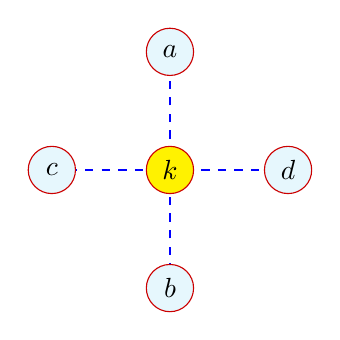
\begin{tikzpicture}[scale=1, font=\normalsize]
			\tikzset{
				cblue/.style={circle, draw=red!80!black, fill=cyan!10, minimum size=6mm, inner sep=1pt},
				cyellow/.style={circle, draw=red!80!black, fill=yellow, minimum size=6mm, inner sep=1pt}
			}
			\draw[dashed, blue, thick] (-1.5,0) -- (1.5,0);
			\draw[dashed, blue, thick] (0,-1.5) -- (0,1.5);
			\node[cblue] at (0,1.5) {$a$};
			\node[cblue] at (0,-1.5) {$b$};
			\node[cblue] at (-1.5,0) {$c$};
			\node[cblue] at (1.5,0) {$d$};
			\node[cyellow] at (0,0) {$k$};
		\end{tikzpicture}
	}
	\par
	\shortans[0]{144}
	\loigiai{
		\begin{itemize}
			\item Ta phân tập $X$ thành các tập sau:
			\begin{itemize}
				\item $X_0 = \{1; 3; 5; 7; 9; 11; 13; 15; 17; 19\}$ (các số ở dạng $y \cdot 2^0$, với $y$ không chia hết cho $2$).
				\item $X_1 = \{2; 6; 10; 14; 18\}$ (các số ở dạng $y \cdot 2^1$, với $y$ không chia hết cho $2$).
				\item $X_2 = \{4; 12; 20\}$ (các số ở dạng $y \cdot 2^2$, với $y$ không chia hết cho $2$).
				\item $X_3 = \{8\}$ (các số ở dạng $y \cdot 2^3$, với $y$ không chia hết cho $2$).
				\item $X_4 = \{16\}$ (các số ở dạng $y \cdot 2^4$, với $y$ không chia hết cho $2$).
			\end{itemize}
			\item Ta có $abk = x \cdot 2^{a'} \cdot 2^{b'} \cdot 2^{k'} = x \cdot 2^{a'+b'+k'}$ và $cdk = y \cdot 2^{c'} \cdot 2^{d'} \cdot 2^{k'} = y \cdot 2^{c'+d'+k'}$ chia hết cho $256$.\\ 
			Suy ra $a'+b'+k'$ và $c'+d'+k'$ lớn hơn hoặc bằng $8$.\\ Với các số $a'$, $b'$, $c'$, $d'$, $k' \in \{0;1;2;3;4\}$.
		\end{itemize}
		Ta có các trường hợp sau:
		\begin{itemize}
			\item \textbf{Trường hợp 1:} Số $k \in X_0 \Rightarrow k'=0 \Rightarrow a'+b'$, $c'+d' \ge 8$. Không tồn tại cặp nào thoả mãn.
			\item \textbf{Trường hợp 2:} Số $k \in X_1 \Rightarrow k'=1 \Rightarrow a'+b'$, $c'+d' \ge 7$. Chỉ tồn tại một bộ $4+3$ không đủ điền. Nên trường hợp này không thoả mãn.
			\item \textbf{Trường hợp 3:} Số $k \in X_2 \Rightarrow k'=2 \Rightarrow a'+b'$, $c'+d' \ge 6$. Chỉ tồn tại các bộ $4+3$, $4+2$, $3+3$, mà chỉ có $1$ số trong mỗi tập $X_3$, $X_4$ nên không đủ chọn ra hai bộ. Nên trường hợp này không thoả mãn.
			\item \textbf{Trường hợp 4:} Số $k \in X_3 \Rightarrow k'=3 \Rightarrow a'+b'$, $c'+d' \ge 5$. Tồn tại các bộ $4+2$, $4+1$, $3+3$, $3+2$. Nhưng chỉ có $1$ số của tập $X_4$ và không còn số nào trong tập $X_3$ nên không đủ chọn hai bộ để điền. Nên trường hợp này không thoả mãn.
			\item \textbf{Trường hợp 5:} Số $k \in X_4 \Rightarrow k'=4 \Rightarrow a'+b', c'+d' \ge 4$. Tồn tại các bộ $3+1$, $3+2$, $2+2$.
			\begin{itemize}
				\item Có một cách chọn $k$ ($1$ cách chọn ra $k=16$).
				\item \textbf{Khả năng 1:} Chọn các bộ dạng $(3+2)$ và $(2+2)$. Chọn ra $1$ số từ $X_3$, chọn ra $1$ số từ $X_2$, để được một cặp. Chọn hai số còn lại từ $X_2$ ta sẽ được cặp nữa. Ta có số cách chọn khả năng này là $\mathrm{C}_1^1 \cdot \mathrm{C}_3^1 \cdot \mathrm{C}_2^2 \cdot 2! \cdot 2! \cdot 2!$ (cách).
				\item \textbf{Khả năng 2:} Chọn các bộ dạng $(3+1)$ và $(2+2)$. Chọn ra $1$ số từ $X_3$, chọn ra $1$ số từ $X_1$, để được một cặp. Chọn hai số của $X_2$ để được hai cặp. Ta có số cách chọn khả năng này là $\mathrm{C}_1^1 \cdot \mathrm{C}_5^1 \cdot \mathrm{C}_3^2 \cdot 2! \cdot 2! \cdot 2!$ (cách).
				\item Suy ra trường hợp này có tất cả số cách xếp là $\mathrm{C}_1^1 \cdot \mathrm{C}_3^1 \cdot \mathrm{C}_2^2 \cdot 2! \cdot 2! \cdot 2! + \mathrm{C}_1^1 \cdot \mathrm{C}_5^1 \cdot \mathrm{C}_3^2 \cdot 2! \cdot 2! \cdot 2! = 144$.
				\item Việc nhân thêm $2! \cdot 2! \cdot 2!$ là ta hoán vị $2$ bộ $ab$ và $cd$ cho nhau, trong mỗi bộ ta tự hoán vị hai vị trí cho nhau.
			\end{itemize}
		\end{itemize}
		Vậy có tất cả $T = 144$ cách chọn.
	}
\end{ex}
%%%=============================%%%
\Closesolutionfile{ans}

\newpage
\indapan{12}{ans/ansTN-Dung}
\indapan[TF]{2}{ans/ansTN-DungSai}
\indapan[SA]{6}{ans/ansTN-DienKhuyet}
%%%%%%%%%%%%%%
%%nhãn kết thúc đề (để đếm số trang tự động mỗi đề)
\label{B\thedeso}